%
\documentclass[%
 reprint,
 amsmath,amssymb,
 aps,
]{revtex4-1}

\usepackage{graphicx}% Include figure files
\usepackage{dcolumn}% Align table columns on decimal point
\usepackage{bm}% bold math


\begin{document}


\title{Comparación Business Intelligence vs Business Analytics}
\author{Yaneth Virginia Aquino Huallpa}
\author{Yofer Nain Catari Cabrera}
\author{Orlando Antonio Acosta Ortiz}
\author{Edward Apaza Mamani}

\affiliation{%
 Universidad Privada de Tacna \textbackslash Facultad de Ingenieria \textbackslash Escuela Profesional de Ingenieria de Sistemas
}%

\begin{abstract}
\begin{center}
\textbf{Resumen}
\end{center}

Business Intelligence ofrece un amplio conjunto de beneficios que impulsan un retorno significativo y tangible
inversión. Elimina la complejidad de convertir datos sin procesar en inteligencia empresarial significativa al dar a las organizaciones el poder de transformar datos de múltiples fuentes en precisos y Permite a los usuarios
tomar decisiones empresariales informadas de forma rápida y segura proporcionando la consulta y los informes
herramientas que necesitan para encontrar, compartir, administrar, publicar y analizar información. El objetivo de los negocios
La inteligencia es permitir que la administración tome decisiones más inteligentes sobre la base del conocimiento
extractos de los datos.

\textbf{Palabras clave:}  Inteligencia de Negocios, toma de decisiones empresariales, análisis, memoria, monitoreo.\\
\begin{center}
\textbf{Abstract}
\end{center}
Business Intelligence offers a broad set of benefits that drive a meaningful and tangible return
investment. Eliminates the complexity of converting raw data into meaningful business intelligence by giving organizations the power to transform data from multiple sources into accurate and allows users
make informed business decisions quickly and safely providing consultation and reports
tools they need to find, share, manage, publish and analyze information. The business objective
Intelligence is to allow management to make smarter decisions based on knowledge
data extracts.
\\

\textbf{Keywords:}  Business Intelligence, business decision making, analysis, memory, monitoring.\\
\end{abstract}

\maketitle


%\tableofcontents

%-----------------------------------------------------------------
\section {Introducción}\label{sec:1}

En los últimos años, el Business Intelligence se ha visto marcado por una evolución que lo destaca como un mercado maduro: \\
- Se ha producido una consolidación del mercado mediante la compra de empresas pequeñas por parte de los principales agentes del mercado (SAP,IBM, Microsoft y Oracle). \\
- Se ha enriquecido con soluciones de codigo abierto que cubren las necesidades de una organización para la explotación de la información.\\
- Han aparecido nuevas empresas con foco en la innovación cubriendo nuevos nichos en el mercado de la inteligencia de negocio como la visualización, el análisis predictivo, las virtual appliances y/o el real-time Business Intelligence.\\
- A pesar de la crisis económica (2008), el mercado de inteligencia de negocio sigue en una fase de crecimiento estable al posicionarse como una necesidad crítica para toda organización.\cite{ref1}\\\\

Business Intelligence nace de la necesidad de las organizaciones para transformar la información en conocimiento, y permitir en forma precisa y eficaz la toma de decisiones\cite{ref3}.El término BI se utilizó a partir del año 1958 por Hans Peter Luhn, quien define BI como: \\
“La capacidad de comprender las interrelaciones de los hechos presentados en tal forma como para orientar la acción hacia una meta deseada” (Luhn, 1958).\cite{ref4} \\
El objetivo básico de la Business Intelligence es apoyar de forma sostenible
y continuada a las organizaciones para mejorar su competitividad, facilitando la información necesaria para la toma de decisiones. El primero que
acuñó el término fue Howard Dresner que, cuando era consultor de Gartner, popularizó Business Intelligence o BI como un término paraguas para describir un conjunto de conceptos y métodos que mejoraran la toma de
decisiones, utilizando información sobre que había sucedido (hechos).\cite{ref2} \\\\

%-----------------------------------------------------------------
\section{Marco Teórico}\label{sec:2}
\subsection{Business Intelligence}
	          \begin{itemize}
                    \item Business Intelligence es el conjunto de metodologías, aplicaciones y tecnologías que permiten reunir, depurar y transformar datos de los sistemas transaccionales e información desestructurada  en información estructurada, para su explotación directa  o para su análisis y conversión en conocimiento, dando así soporte a la toma de decisiones sobre el negocio.\cite{Oracle}
\\

La inteligencia de negocio Actúa como un factor estratégico para una empresa u organización, generando una potencial ventaja competitiva, que no es otra que proporcionar información privilegiada para responder a los problemas de negocio: entrada a nuevos mercados, promociones u ofertas de productos, eliminación de islas de información, control financiero, optimización de costes, planificación de la producción, análisis de perfiles de clientes, rentabilidad de un producto concreto, etc.

Los principales productos de Business Intelligence que existen hoy en día son:

-  Cuadros de Mando Integrales (CMI)

-  Sistemas de Soporte a la Decisión (DSS)

-  Sistemas de Información Ejecutiva (EIS)
	          \end{itemize}
\subsection{Aplicaciones de  Business Intelligence }
Las herramientas de inteligencia de negocio son aplicaciones digitales diseñadas para colaborar con el Business Intelligence durante el análisis y la presentación de datos.\\
La Inteligencia de Negocios o Business Intelligence (BI) permite a las compañías contar con la información adecuada para una mejor toma de decisiones.  Las compañías que implementan el BI logran sacar mayor provecho de las situaciones de crisis gracias a la posibilidad de contar con un análisis de mercado más acertado debido a que los datos pesados son transformados en importantes estrategias corporativas.
Actualmente, las herramientas de BI disponibles en el mercado son incontables, pero estas 20 no pueden pasar desapercibidas:
\begin{itemize}
\item Microsoft Dynamics NAV\\
Especial para pequeñas y medianas empresas que buscan mejorar su competitividad.
\item  Microsoft Dynamics CRM\\
Efectiva para la administración de clientes.
\item Oracle Business Intelligence\\
Una de las más completas en el mercado ya que cuenta con paneles interactivos, análisis predictivos en tiempo real, entre otros.
\item Ultimus\\
Un entorno integrado que permite compartir información entre aplicaciones.
\item  Office SharePoint Server\\
Facilita el acceso a la información en cualquier momento y lugar.
\item QlikView\\
Mantiene las bases de datos al alcance de una manera sin precedentes.
\item Microsoft Performance Point Server\\
Permite supervisar, alinear y hacer un plan de negocio.
\item  Microsoft SQL Server\\
Adecuada para realizar un análisis panorámico de la empresa y tomar las mejores decisiones.
\item  JetReports\\
Especial para crear informes ERP.
\item Eclipse BIRT Project\\
Genera informes para aplicaciones web de código abierto.
\item  JasperReports\\
Permite crear informes de rápida impresión.
\item  LogiReport\\
Aplicación gratuita basada en web de LogiXML
\item OpenI\\
Aplicación web orientada al reporting OLAP.
\item  SPSS\\
Programa estadístico especialmente empleado en ciencias sociales e investigaciones de mercado.
\item  Pentaho\\
Incluye herramientas para generar informes, minería de datos, ETL, entre otros.
\item  RapidMiner\\
Permite analizar datos a través de un entorno gráfico.
\item  Crystal Reports\\Genera informes desde bases de datos múltiples.
\item  ApeSoft\\Ofrece una interface sencilla similar a Microsoft Excel.
\item  SAS Institute\\Facilita la gestión de riesgo financiero, desarrollo de modelos de minería de datos, etc.
\item  NiMbox\\Organiza los datos de la empresa en interactivas aplicaciones.
 \end{itemize}
\subsection{Business Analytics}
	          \begin{itemize}
		\item  Es el conjunto de métodos y técnicas utilizadas para trabajar como enlace entre los stackeholders, con el fin de comprender la estructura, políticas y operaciones de una organización y recomendar soluciones que permitan a la organización alcanzar sus objetivos .\cite{Oracle1}
	           \end{itemize}
\subsection{Aplicaciones de  Business Analitycs }
Toda empresa necesita un plan de negocio. Muchos emprendedores caen en la tentación de poner en marcha su negocio sin analizar nada previamente y se limitan a cruzar los dedos esperando que salga bien. Y podría ser que sí, pero lo más probable es que no.\\
Lo ideal es llevar a cabo un análisis previo pormenorizado del sector y el mercado en el que pensamos adentrarnos. Hay numerosas herramientas de análisis estratégico gratuitas que nos pueden servir para para identificar qué distingue nuestra marca del resto y elaborar un buen plan de negocio para nuestra futura empresa. Estas son algunas de ellas.  
\begin{itemize}
\item Análisis PEST
\\Con esta herramienta de análisis estratégico podremos analizar el entorno en el que queremos crear o establecer nuestra empresa, negocio o proyecto. Nos permite identificar posibles cambios de escenario en nuestro sector o en la región para detectar y aprovechar posibles oportunidades de crecimiento. El nombre es un acrónimo de cuatro factores:

Políticos: estabilidad política, la posibilidad de un cambio de gobierno que de lugar a cambios en las políticas fiscales o en materia de subvenciones, posibles cambios en los tratados comerciales, existencia o no de grupos de presión.
Económicos: economía en crecimiento o en recesión, tendencia del consumo, situación de confianza o de inestabilidad, los tipos de cambio, el nivel de inflacción…
Socioculturales: hábitos sociales, cambios en los gustos o en las modas de la gente, formas de comunicación habituales, demografía, salud, valores.
Tecnológicos: tecnología actual, posibles avances, desarrollos en marcha, conocimientos, inversión en I+D, información.
Debemos analizar en qué medida cada uno de estos factores macroambientales podría influir positiva o negativamente en nuestra empresa.  
\item Análisis PESTEL
\\Es una variación del anterior que añade dos factores más a los cuatro del análisis PEST. Además de tener en cuenta los factores políticos, económicos, sociales y tecnológicos, se analizarán también los factores:

Ecológicos: por ejemplo, el cambio climático puede tener consecuencias en diversos sectores como el turístico o el de las aseguradoras. Las leyes de protección medioambiental o las regulaciones en materia de gestión de residuos o de energías también pueden influir en una empresa.
Legales: leyes contra la discriminación, leyes de defensa del consumidor, leyes antimonopolio, licencias, legislación laboral, leyes de protección de la salud, sectores con una protección especial.
\item Análisis FODA:
\\Es una herramienta de análisis estratégico que nos permite analizar la situación interna y externa de una empresa o proyecto. Es como hacer una fotografía de la situación de nuestra empresa. Por eso, dado que esta situación no es estático, sino que evoluciona continuamente a lo largo del tiempo, además de utilizarlo para elaborar el plan de negocio de nuestra empresa, es bueno repetirlo posteriormente cada cierto tiempo. El objetivo es conocer la situación real en la que se encuentra la organización, empresa o proyecto en cada momento y, en función de ello, planear la estrategia de futuro más adecuada. El nombre de esta herramienta de análisis es un acrónimo de Fortalezas, Oportunidades, Debilidades y Amenazas. 

\item Las 5 fuerzas de Porter:\\
Esta herramienta de análisis estratégico. El modelo delimita un marco que nos permite analizar el nivel de competencia dentro de un sector para poder idear, así, una estrategia de negocio que haga rentable nuestra empresa. En este sentido, es ideal para elaborar un plan de negocio, dado que es fundamental analizar la competencia antes de crear una empresa, por lo que este modelo es especialmente interesante para emprendedores. Las cinco fuerzas de Porter son las siguientes:

- Poder de negociación de los compradores o clientes
- Poder de negociación de los proveedores o vendedores
- Amenaza de nuevos competidores
- Amenaza de productos sustitutos
- Rivalidad entre los competidores

\item Estrategia del océano azul:\\
Esta herramienta, más que para elaborar nuestro plan de negocio, es ideal para hacernos pensar y ver cómo queremos enfocar nuestra empresa. Una estrategia de océano azul es lo que puede llevar nuestra empresa al éxito. Por eso todo emprendedor debería conocer esta herramienta y, antes de montar su empresa soñada, dedicar un tiempo a pensar cuál puede ser su estrategia del océano azul.	
\item Modelo de las 7 S:
\\A diferencia de la mayoría de las herramientas de análisis estratégico que suelen centrarse en el análisis externo, El modelo analiza, concretamente, 7 factores.

- Estrategia (Strategy)\\
- Estructura (Structure)\\
- Sistemas (Systems)\\
- Estilo (Style)\\
- Valores compartidos (Shared values)\\
- Personal (Staff)\\
- Habilidades (Skills)
La idea del modelo es que las organizaciones no operan como un conjunto de silos estancos, sino más bien como una red de piezas interconectadas. Por eso es fundamental que los siete factores recogidos en el modelo estén alineados para que nuestra empresa tenga éxito.
	\end{itemize} 

\subsection{Diferencia entre Business Intelligence y Business Analytics}
	     \begin{itemize}
		\item Business Intelligence es el proceso que comprende tecnologías y estrategias incorporadas por las industrias empresariales para analizar los datos comerciales existentes que proporcionan eventos pasados históricos, actuales y predictivos de las operaciones comerciales.
La inteligencia empresarial y el análisis son soluciones de gestión de datos implementadas en empresas y empresas para recopilar datos históricos y actuales, al tiempo que utilizan estadísticas y software para analizar información en bruto y ofrecer información para tomar mejores decisiones futuras.

		\item Business Analytics es el proceso de las tecnologías y estrategias utilizadas para continuar explorando y extraer los conocimientos y el rendimiento de la información comercial pasada para impulsar una planificación comercial futura exitosa.
Business analytics (BA) se refiere a las habilidades, tecnologías, prácticas para la exploración iterativa continua y la investigación del desempeño comercial anterior para obtener información y conducir la planificación comercial.
\cite{Educba}
	           \end{itemize}
\subsection{Comparación entre Business Intelligence vs Business Analytics}
  \begin{itemize}
		\item Business Analytics es el proceso de las tecnologías y estrategias utilizadas para continuar explorando y extraer los conocimientos y el rendimiento de la información comercial pasada para impulsar una planificación comercial futura exitosa.\cite{Educba}
\begin{center}
		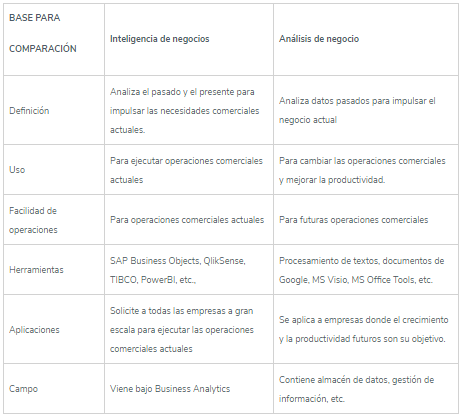
\includegraphics[width=9cm]{./Imagenes/3}
		\end{center}
	           \end{itemize}
%-----------------------------------------------------------------
\section{Análisis}\label{sec:3}
	\begin{itemize}
		\item Cada organización tiene la necesidad de análisis e inteligencia de negocios. Es decir, cada organización tiene datos que necesitan para recopilar, analizar e interpretar. A medida que la tecnología evoluciona y la cantidad de datos y fuentes de datos crecen exponencialmente.
		\item Business Intelligence analiza datos pasados y presentes para operar el negocio acual de manera eficiente,mientras que Business Analytics analiza los datos pasados para analizar escenarios actuales y estar preparado para los negocios futuros.

                     \item Elegir las soluciones para el negocio depende de los objetivos, metas y objetivos de la empresa. Las empresas que requieren grandes cantidades de datos en casos de almacenamiento de datos y grandes informes visuales impactantes deben considerar seriamente la inteligencia empresarial como su herramienta para operar sus negocios de manera productiva.
	\end{itemize}
\section{Conclusiones}\label{sec:4}
\begin{itemize}
\item La  gran mayoría de empresas no utilizan sistemas de inteligencia empresarial para gestionar sus negocios. Estas herramientas son muy enriquecedoras para la gestión actual, a lo que añaden las siguientes ventajas para el  uso de Software de Inteligencia de Negocios:

 a)  Los sistemas de Business Intelligence ayudan a hacer más competitiva la estrategia de la empresa.

 b)  Apoyan la toma de decisiones que son vitales para obtener mejores resultados.

 c)   La Inteligencia de Negocios facilita notablemente la interactividad entre usuarios, clientes y proveedores.

 d)   Facilitan el acceso a los datos críticos de la empresa y las informaciones corporativas para la integración de datos y la toma de decisiones

 e)  Permite alinear acciones de diferentes departamentos e igualmente ayuda a controlar cada línea de negocio o departamento con métricas específicas.
 \\
\end{itemize} 
% Bibliografia.
%-----------------------------------------------------------------
\bibliographystyle{plain}
\bibliography{Bibliografia}

\end{document}
